% !TeX root = main.tex
% !TEX program = pdflatex

% =============================================================
% CAPÍTULO 11 — ESQUELETO (pendiente de redactar)
% Mapea con el descriptor oficial: RA8 (Diseñar un sistema de
% instrumentación... con instrumentación programable y virtual,
% procesando la información disponible).
% Curso de Telecomunicaciones: priorizar ejemplos de banco de laboratorio
% de RF/óptica (analizador de espectros, fuente óptica, multímetro de
% precisión) frente a ejemplos de automatización industrial.
% =============================================================

\chapter{Instrumentación Virtual y Programable}\label{cap:instrumentacion_virtual}

Hasta aquí, el final de la cadena de medida era un número en el registro de un convertidor (Capítulo~\ref{cap:daq}) o un dato que viajaba por un bus (Capítulo~\ref{cap:buses}). En un banco de laboratorio real, sin embargo, la mayoría de las medidas no se hacen con un sensor propio y una tarjeta de adquisición, sino con \emph{instrumentos}: un multímetro de precisión, un generador de funciones, un osciloscopio, un analizador de espectros, un medidor de potencia óptica. Cada uno de ellos contiene ya, dentro de su caja, toda la cadena que hemos estudiado --la sonda o el sensor, el acondicionamiento, la conversión y, casi siempre, el cálculo--, y el ingeniero se limita a leer su pantalla.

Durante décadas ese diálogo ha sido manual: se gira un mando, se espera a que la lectura se estabilice, se anota el valor y se repite el proceso en el punto siguiente. El modelo aguanta mientras la medida es puntual, pero se vuelve insostenible en cuanto hay que repetirla muchas veces --un barrido de frecuencia de cientos de puntos, una campaña de medida de días, una batería de ensayos con varios instrumentos a la vez--, y desperdicia la capacidad de cálculo de la máquina sobre la que se está anotando. La alternativa es la instrumentación \emph{programable} y \emph{virtual}: instrumentos con una interfaz de control remoto, normalmente un bus digital, sobre la que un ordenador puede escribir y leer, y un software que sustituye al panel frontal, al cuaderno de laboratorio y, en muchos casos, a buena parte del propio instrumento~\cite{johnson2006labview}. Este capítulo recorre ese camino: qué es y qué aporta la instrumentación virtual (Sección~\ref{sec:instrumentacion_virtual}), con qué buses y con qué lenguaje se dialoga con los instrumentos (Sección~\ref{sec:scpi}), cómo se escribe una medida automatizada paso a paso (Sección~\ref{sec:pyvisa}) y qué lugar ocupan los entornos gráficos de programación (Sección~\ref{sec:labview}).

\section{El Concepto de Instrumentación Virtual}\label{sec:instrumentacion_virtual}

La idea que hay detrás de la instrumentación virtual es sencilla: separar el instrumento en dos mitades y quedarse con lo mejor de cada una. La primera mitad es el hardware --la sonda o el sensor, el acondicionamiento y el convertidor--, que es donde reside la calidad metrológica de la medida: su resolución, su exactitud y sus límites son los que estudiamos en el Capítulo~\ref{cap:metrologia}, y no mejoran por el hecho de conectarlo a un ordenador. La segunda mitad es todo lo demás --la presentación del resultado, el control de la medida, su registro y su procesado--, y esa mitad se traslada al ordenador. El panel frontal se convierte en una ventana, los mandos en controles de pantalla y la anotación en un fichero de datos. La Figura~\ref{fig:instrumentacion_virtual} contrasta las dos formas de trabajar.

\begin{marginfigure}
    \centering
    \begin{tikzpicture}[scale=0.8, >=Stealth]
        % ── (a) instrumento de sobremesa ──────────────────────
        \begin{scope}
            \node[anchor=north west, font=\itshape\scriptsize, gray] at (0.0,3.6) {(a) operación manual};
            \draw[thick] (0.0,0.7) rectangle (2.8,3.1);
            \draw[fill=gray!12] (0.3,2.0) rectangle (2.5,2.8);
            \node[font=\tiny] at (1.4,2.4) {12,043 mV};
            \draw (0.6,1.4) circle (0.22);
            \draw (1.4,1.4) circle (0.22);
            \draw (2.2,1.4) circle (0.22);
            \node[font=\tiny, anchor=north] at (1.4,0.65) {panel físico};
            \draw[->] (2.8,1.6) -- (3.5,1.6);
            \draw[thick] (3.5,1.0) rectangle (5.9,2.2);
            \node[font=\tiny, align=center] at (4.7,1.6) {cuaderno de\\laboratorio};
        \end{scope}
        % ── (b) instrumentación virtual ───────────────────────
        \begin{scope}[yshift=-3.6cm]
            \node[anchor=north west, font=\itshape\scriptsize, gray] at (0.0,3.6) {(b) instrumentación virtual};
            \draw[thick] (0.0,0.7) rectangle (1.9,3.1);
            \draw[fill=gray!12] (0.2,2.0) rectangle (1.7,2.8);
            \node[font=\tiny] at (0.95,2.4) {12,043 mV};
            \node[font=\tiny, anchor=north] at (0.95,1.9) {instrumento};
            % bus de control
            \draw[<->, thick] (1.9,1.7) -- (3.5,1.7);
            \node[font=\tiny, align=center, anchor=south] at (2.7,1.75) {bus de\\control};
            % ordenador
            \draw[thick] (3.5,0.7) rectangle (6.4,3.1);
            \node[font=\scriptsize] at (4.95,2.75) {ordenador};
            \node[font=\tiny, align=center] at (4.95,2.05) {panel virtual\\procesado\\registro};
        \end{scope}
    \end{tikzpicture}
    \caption[Operación manual frente a instrumentación virtual.]{Las dos formas de trabajar con un instrumento de laboratorio. \emph{(a)}~En la operación manual, el usuario actúa sobre el panel físico, lee la pantalla y traslada el valor a un cuaderno: la medida no queda registrada en formato utilizable y su repetición depende de la paciencia y de la atención del operador. \emph{(b)}~En instrumentación virtual, el instrumento sigue midiendo, pero el ordenador le envía los comandos por el bus de control y recibe los datos: el panel, el registro y el procesado son software. La calidad de la medida sigue siendo la del instrumento; lo que cambia es cuántas medidas se pueden hacer, con qué repetibilidad y para qué.}\label{fig:instrumentacion_virtual}
\end{marginfigure}

El grado de virtualización no es el mismo en todos los casos, y conviene distinguir tres niveles, resumidos en la Tabla~\ref{tab:niveles_virtual}. En el primero, el ordenador se limita a gobernar un instrumento que ya está completo: un multímetro de banco al que se le pide una lectura tras otra. En el segundo, el hardware es un simple digitalizador --una tarjeta de adquisición o un módulo enchufable-- y la función de medida la construye el software: representar la señal en pantalla, disparar la captura en el instante adecuado, calcular el valor eficaz, obtener el espectro. Es lo que hace un osciloscopio virtual, y es el caso en que el programa es, literalmente, el instrumento. En el tercero, el hardware se reduce a una electrónica de conversión genérica --y, en radiofrecuencia, de traslación de frecuencia-- y es el software quien define qué instrumento se está construyendo: un analizador de espectros no es más que la transformada de Fourier de una banda digitalizada, y el mismo equipo, con otro programa, se convierte en un analizador de redes o en una radio definida por software.

\begin{table}[ht]
    \centering
    \small
    \setlength{\tabcolsep}{3pt}
    \begin{tabularx}{\linewidth}{@{} L{0.19\linewidth} >{\centering\arraybackslash}X >{\centering\arraybackslash}X >{\centering\arraybackslash}X @{}}
        \toprule
        \textbf{Nivel} & \textbf{Papel del hardware} & \textbf{Papel del software} & \textbf{Ejemplo} \\
        \midrule
        Panel virtual & El instrumento completo: sonda, acondicionamiento, conversión y cálculo & La interfaz, la secuencia de medida y el registro & Multímetro de banco con un script de barrido \\
        Instrumento sobre módulos & El digitalizador o la tarjeta de adquisición (Capítulo~\ref{cap:daq}) & La función de medida: representación, disparo, cálculo y análisis & Osciloscopio o analizador de espectros virtual \\
        Instrumento definido por software & Conversión y, si acaso, traslación de frecuencia & Define el instrumento: filtrado, detección, unidades y análisis & Analizador por FFT; radio definida por software \\
        \bottomrule
    \end{tabularx}
    \caption[Tres grados de instrumentación virtual.]{Los tres grados de instrumentación virtual. Cuanto más abajo, más hardware se sustituye por software y más flexible --y también más dependiente del programa-- es el sistema de medida. En los tres casos la exactitud sigue acotada por la parte analógica, que no desaparece.\protect\label{tab:niveles_virtual}}
\end{table}

\marginnote{\textbf{Ejemplo:} un barrido de la respuesta en frecuencia de un filtro con cien puntos exige, a mano, ajustar la frecuencia, esperar la lectura y anotarla: unos \SI{20}{\second} por punto, algo más de media hora de trabajo repetitivo y cien ocasiones de equivocarse al copiar. El mismo barrido programado tarda unas décimas de segundo por punto, medio minuto en total, y deja los datos en un fichero y la gráfica hecha. La diferencia no es de velocidad, sino de que el procedimiento queda escrito y es el mismo cada vez.}

Las ventajas de trabajar así van mucho más allá de ahorrar tiempo. La automatización permite medidas que a mano serían impracticables --barrer una banda completa, promediar miles de capturas, repetir un ensayo durante días--. La repetibilidad mejora porque el procedimiento deja de depender del pulso y de la atención de una persona: el mismo script mide siempre igual, y si otro día hay que repetir la campaña, se ejecuta de nuevo. La trazabilidad mejora también, y quizá sea lo más valioso en un laboratorio: el registro de datos va acompañado de la configuración de los instrumentos, de la fecha y de la versión del programa, de modo que el procedimiento de medida queda documentado junto con el resultado. Y el procesado deja de estar limitado por lo que el instrumento traiga de fábrica: promediado, filtrado, transformada de Fourier, propagación de incertidumbres o comparación con un modelo se hacen en el ordenador, con las herramientas del Capítulo~\ref{cap:metrologia}.

El precio es doble. Por un lado, el ordenador introduce sus propios errores: no es un sistema de tiempo real --su sistema operativo atiende a muchas tareas a la vez-- y los tiempos que controla el software tienen una dispersión de milisegundos, inadmisible si lo que se mide exige precisión de microsegundos. Cuando la cronología importa, hay que dejar el disparo y la sincronización en manos del hardware --la señal de disparo del instrumento, o los mecanismos de sincronización temporal de los buses modernos-- y usar el ordenador solo para lo que hace bien: decidir, guardar y calcular. Por otro lado, el software pasa a formar parte del sistema de medida y hay que tratarlo como tal: versiones, verificación, copias de seguridad y documentación, porque un programa que cambia sin control cambia también la medida. En un laboratorio acreditado, la validación del software no es una recomendación, sino un requisito del mismo rango que la calibración de los instrumentos.

\marginnote{\textbf{Límite práctico:} la instrumentación virtual no mejora la exactitud de ninguna medida; mejora la cantidad de medidas, su repetibilidad y el uso que se hace de ellas. Confundir ambas cosas es el error más frecuente al automatizar un banco: un programa no corrige un instrumento fuera de especificación ni un sensor mal calibrado.}

\section{Buses de Control y el Estándar SCPI}\label{sec:scpi}

Para que un ordenador gobierne un instrumento hacen falta dos acuerdos: uno físico, sobre cómo viajan los bits entre ambos, y otro lógico, sobre qué significan. El primero lo resuelven los buses de control, que en instrumentación tienen una historia propia y bien poblada; el segundo lo resuelve un lenguaje de comandos normalizado, el estándar SCPI. Entre ambos se ha consolidado además una capa de software, VISA, cuya única misión es que el programa de medida no tenga que saber por dónde está conectado el instrumento. Esta sección recorre las tres.

\subsection{Los Buses de Control}\label{sub:buses_control}

El primer bus pensado para instrumentos nació en Hewlett-Packard en los años sesenta --el \emph{HP Interface Bus}-- y se convirtió en norma en 1975 con el nombre de \emph{IEEE 488}, conocida después como \emph{GPIB} (\textsc{general purpose interface bus}). Su diseño explica por qué ha durado tanto: es un bus paralelo de ocho líneas de datos, tres de sincronización y cinco de gestión, con un conector de 24 contactos que se apila, de modo que los instrumentos se encadenan uno tras otro; admite hasta quince aparatos en unos veinte metros de cable, a velocidades del orden del megabyte por segundo, y no transporta solo la información, sino también el protocolo que decide quién habla en cada momento --los papeles de \emph{hablante}, \emph{oyente} y \emph{controlador}--. Con una sola tarjeta GPIB en el ordenador se gobierna, por tanto, todo un banco de laboratorio, y esa es la razón de que siga habiendo instrumentos con puerto GPIB varias décadas después.

A partir de los años noventa, los buses del ordenador fueron desplazándolo. El puerto serie fue el primero en usarse --sencillo y lento, un instrumento por puerto--, y el \emph{USB} lo sustituyó con ventaja a partir de 2003, cuando se definió la clase específica para instrumentación (\textsc{usb test and measurement class, usbtmc}): el mismo modelo de mensajes del GPIB, pero sobre los canales rápidos del USB y con el cable y los conectores que todo el mundo tiene~\cite{usbtmc_2003}. Su limitación es la topología: el USB es punto a punto, de modo que cada instrumento ocupa un puerto --o hay que recurrir a concentradores--. La respuesta más reciente es la red local: en 2005 se publicó el estándar \emph{LXI} (\textsc{lan extensions for instrumentation}), que no define un cable nuevo, sino que convierte al instrumento en un nodo más de la red Ethernet, con su dirección IP, su servidor web para identificarlo y configurarlo, y un conjunto de protocolos de medida sobre TCP/IP~\cite{lxi_2016}. La ventaja es evidente: la distancia deja de ser un problema, un conmutador conecta a tantos instrumentos como puertos tenga, y la sincronización temporal entre equipos --necesaria cuando varias medidas deben referirse al mismo instante-- se resuelve con los mecanismos de tiempo de la propia red. La Tabla~\ref{tab:buses_instrumentacion} compara las alternativas, y la Figura~\ref{fig:buses_instrumentacion} contrapone las dos topologías dominantes.

\begin{marginfigure}
    \centering
    \begin{tikzpicture}[scale=0.8, >=Stealth]
        % ── (a) GPIB en cadena ────────────────────────────────
        \begin{scope}
            \node[anchor=north west, font=\itshape\scriptsize, gray] at (0.0,3.0) {(a) GPIB: en cadena};
            \draw[thick] (0.0,1.7) rectangle (1.4,2.5);
            \node[font=\scriptsize] at (0.7,2.1) {PC};
            \draw[line width=1.5pt] (1.4,2.1) -- (6.2,2.1);
            \node[font=\tiny, anchor=south west] at (1.6,2.15) {bus GPIB (24 hilos)};
            \draw (2.9,2.1) -- (2.9,1.6);
            \draw (5.1,2.1) -- (5.1,1.6);
            \node[circ] at (2.9,2.1){}; \node[circ] at (5.1,2.1){};
            \draw[thick] (2.2,0.6) rectangle (3.6,1.6);
            \node[font=\tiny] at (2.9,1.1) {instrumento};
            \draw[thick] (4.4,0.6) rectangle (5.8,1.6);
            \node[font=\tiny] at (5.1,1.1) {instrumento};
            \node[gray, font=\tiny, anchor=north west] at (0.0,0.45) {hasta 15 instrumentos, 20 m, $\approx$\SI{1}{\mega\byte\per\second}};
        \end{scope}
        % ── (b) LXI en red ────────────────────────────────────
        \begin{scope}[yshift=-3.7cm]
            \node[anchor=north west, font=\itshape\scriptsize, gray] at (0.0,3.7) {(b) LXI: en red};
            \draw[thick] (0.0,1.9) rectangle (1.4,2.7);
            \node[font=\scriptsize] at (0.7,2.3) {PC};
            \draw (1.4,2.3) -- (2.2,2.3);
            \draw[thick] (2.2,2.0) rectangle (3.6,2.6);
            \node[font=\tiny] at (2.9,2.3) {conmutador};
            \draw (3.6,2.5) -- (4.0,2.5) -- (4.0,3.1) -- (4.4,3.1);
            \draw (3.6,2.1) -- (4.0,2.1) -- (4.0,1.3) -- (4.4,1.3);
            \draw[thick] (4.4,2.7) rectangle (5.9,3.5);
            \node[font=\tiny] at (5.15,3.1) {instrumento};
            \draw[thick] (4.4,0.9) rectangle (5.9,1.7);
            \node[font=\tiny] at (5.15,1.3) {instrumento};
            \node[gray, font=\tiny, anchor=north west] at (0.0,0.5) {cada instrumento es un nodo de la red, con su dirección IP};
        \end{scope}
    \end{tikzpicture}
    \caption[Topologías de los buses de control: GPIB en cadena y LXI en red.]{Las dos topologías que dominan el control de instrumentos. \emph{(a)}~GPIB es un bus paralelo en el que los instrumentos se encadenan con conectores apilables: una sola tarjeta en el ordenador gobierna hasta quince aparatos dentro de los veinte metros de cable que admite el bus. \emph{(b)}~En LXI el instrumento es un nodo de la red Ethernet: se conecta a un conmutador, tiene su dirección IP y su propio servidor web, y el límite de distancia pasa a ser el de la red.}\label{fig:buses_instrumentacion}
\end{marginfigure}

\begin{table}[ht]
    \centering
    \small
    \setlength{\tabcolsep}{3pt}
    \forceversofloat % la tabla cae en página par (verso); sin forzar, el caption sale al lado contrario
    \begin{tabularx}{\linewidth}{@{} L{0.24\linewidth} >{\centering\arraybackslash}X >{\centering\arraybackslash}X @{}}
        \toprule
        \textbf{Bus} & \textbf{Medio y alcance} & \textbf{Velocidad y número de instrumentos} \\
        \midrule
        GPIB (IEEE 488) & Cable paralelo de 24 hilos; hasta 20 m en cadena & En torno a \SI{1}{\mega\byte\per\second}; hasta 15 instrumentos \\
        USB (USBTMC) & Cable USB; unos metros & Alta; un instrumento por puerto \\
        Ethernet (LXI) & Red local: el alcance lo fija la red & Alta; muchos instrumentos por conmutador, con sincronización temporal \\
        Serie (RS-232) & Cable serie; pocos metros & Baja; un instrumento por puerto \\
        Módulos (PXI, VXI) & Chasis con bus de alta velocidad & Muy alta, con sincronización entre módulos \\
        \bottomrule
    \end{tabularx}
    \caption[Comparación de los buses de control de instrumentos.]{Comparación de los buses de control de instrumentos. El GPIB, diseñado para encadenar aparatos en un banco, sigue siendo el más común en el instrumental antiguo; el USB ha ocupado su lugar en los equipos nuevos, y Ethernet lo desplaza cuando hay que reunir muchos instrumentos o separarlos por distancias grandes.\protect\label{tab:buses_instrumentacion}}
\end{table}

\subsection{La Capa de Abstracción: VISA}\label{sub:visa}

Con cinco formas de conectar un instrumento, el programa de medida correría el riesgo de depender del cable: un código escrito para un multímetro GPIB no serviría para el mismo multímetro con interfaz USB, aunque las medidas fuesen idénticas. Para evitarlo, la alianza VXIplug\&play --hoy integrada en la IVI Foundation-- publicó en 1995 la especificación \emph{VPP-4.3: The VISA Library}, que define la \emph{arquitectura de software de instrumentos virtuales} (\textsc{virtual instrument software architecture, visa})~\cite{visa_vpp43}. VISA es una interfaz de programación única para todos los buses: el programa abre una \emph{sesión} con el instrumento, le escribe comandos, lee respuestas y la cierra, sin que en ninguna de esas operaciones aparezca el tipo de conexión.

Lo único que cambia de un bus a otro es la dirección con la que se identifica al instrumento, la cadena de recurso, que es distinta para cada medio y sigue una sintaxis regular: \texttt{GPIB0::22::INSTR} para el instrumento de dirección 22 del bus GPIB, \texttt{USB0::0x0957::0x0607::serie::INSTR} para uno conectado por USB --donde los números hexadecimales identifican al fabricante y al modelo--, \texttt{TCPIP0::192.168.1.50::INSTR} para un instrumento en red y \texttt{ASRL1::INSTR} para uno conectado al puerto serie. Cambiar de bus se reduce así a cambiar esa cadena: el resto del programa no se toca. Sobre VISA se apoyan además los controladores de instrumento, que empaquetan los comandos concretos de cada modelo en funciones con nombre --``medir tensión continua''-- y añaden la posibilidad de intercambiar instrumentos equivalentes de distintos fabricantes sin reescribir el programa.

Conviene retener dos consecuencias prácticas de esta arquitectura. La primera es que VISA es una norma de interfaz, no un producto: cada fabricante publica su propia implementación --NI-VISA, Keysight VISA y otras-- y el programa es portable, pero la instalación no es idéntica en todos los ordenadores. La segunda es que en una misma máquina no deben convivir dos implementaciones completas de VISA, porque ambas quieren controlar los mismos recursos; de ahí que los instaladores modernos compartan componentes comunes en lugar de duplicarlos.

\subsection{El Estándar SCPI}\label{sub:scpi}

Falta el lenguaje. Hasta los años noventa, cada fabricante definía los comandos de sus instrumentos y el mismo programa había que reescribirlo al cambiar de marca; las propias normas IEEE 488.2 habían dado un primer paso al normalizar los códigos, los formatos y los llamados \emph{comandos comunes} --los que empiezan por asterisco--, pero no el vocabulario de las medidas. En 1990, y en su revisión vigente de 1999, el consorcio SCPI publicó el estándar \emph{SCPI} (\textsc{standard commands for programmable instruments}), que define ese vocabulario sobre la parte de la norma IEEE 488.2 que no depende del bus~\cite{ieee488_2_1992,scpi_1999}.

La sintaxis de SCPI es un árbol jerárquico cuyas ramas se separan con dos puntos. Un comando es un camino desde la raíz, y cada nivel precisa el significado del anterior: \texttt{:MEASure:VOLTage:DC?} pide una medida de tensión continua, \texttt{:SOURce:FREQuency} fija la frecuencia de un generador y \texttt{:SENSe:FREQuency:SPAN} el margen de frecuencias de un analizador de espectros. La Figura~\ref{fig:scpi_arbol} muestra esa estructura. Dos reglas hacen el lenguaje cómodo de escribir: cada palabra puede abreviarse a sus letras mayúsculas --\texttt{:MEASure} admite \texttt{:MEAS}, \texttt{:VOLTage} admite \texttt{:VOLT}--, y después de un punto y coma el siguiente comando continúa en la misma rama, de modo que \texttt{:SENSe:FREQuency:STARt 1E6;STOP 1E9} fija el principio y el final del barrido sin repetir el camino. El signo de interrogación convierte cualquier comando en una consulta, y su respuesta es el dato.

\begin{marginfigure}
    \centering
    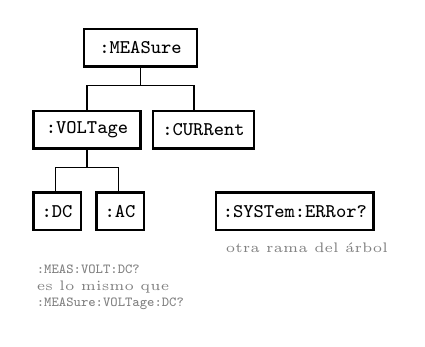
\begin{tikzpicture}[scale=0.8]
        % rama :MEASure
        \draw[thick] (0.9,4.3) rectangle (2.7,4.9);
        \node[font=\ttfamily\scriptsize] at (1.8,4.6) {:MEASure};
        \draw (1.8,4.3) -- (1.8,4.0);
        \draw (0.95,4.0) -- (2.65,4.0);
        \draw (0.95,4.0) -- (0.95,3.6);
        \draw (2.65,4.0) -- (2.65,3.6);
        \draw[thick] (0.1,3.0) rectangle (1.8,3.6);
        \node[font=\ttfamily\scriptsize] at (0.95,3.3) {:VOLTage};
        \draw[thick] (2.0,3.0) rectangle (3.6,3.6);
        \node[font=\ttfamily\scriptsize] at (2.8,3.3) {:CURRent};
        \draw (0.95,3.0) -- (0.95,2.7);
        \draw (0.45,2.7) -- (1.45,2.7);
        \draw (0.45,2.7) -- (0.45,2.3);
        \draw (1.45,2.7) -- (1.45,2.3);
        \draw[thick] (0.1,1.7) rectangle (0.85,2.3);
        \node[font=\ttfamily\scriptsize] at (0.475,2.0) {:DC};
        \draw[thick] (1.1,1.7) rectangle (1.85,2.3);
        \node[font=\ttfamily\scriptsize] at (1.475,2.0) {:AC};
        % rama :SYSTem
        \draw[thick] (3.0,1.7) rectangle (5.5,2.3);
        \node[font=\ttfamily\scriptsize] at (4.25,2.0) {:SYSTem:ERRor?};
        \node[gray, font=\tiny, anchor=north west] at (3.0,1.65) {otra rama del árbol};
        % nota de abreviaturas
        \node[gray, font=\tiny, anchor=north west, align=left] at (0.0,1.3) {\texttt{:MEAS:VOLT:DC?}\\ es lo mismo que\\ \texttt{:MEASure:VOLTage:DC?}};
    \end{tikzpicture}
    \caption[Árbol de comandos SCPI.]{Estructura en árbol de los comandos SCPI. Cada comando es un camino desde la raíz y cada nivel precisa al anterior: la raíz \texttt{:MEASure} pide una medida, \texttt{:VOLTage} la magnitud y \texttt{:DC} el tipo. Las mayúsculas de cada palabra son la abreviatura permitida, de modo que la consulta \texttt{:MEAS:VOLT:DC?} significa lo mismo que \texttt{:MEASure:VOLTage:DC?}. La segunda rama, \texttt{:SYSTem:ERRor?}, es la que devuelve el primer error acumulado en la cola del instrumento, y los comandos que empiezan por asterisco son comunes a todos los aparatos.}\label{fig:scpi_arbol}
\end{marginfigure}

Los comandos comunes merecen una mención aparte, porque son los que permiten escribir programas genéricos. \texttt{*IDN?} devuelve la identificación del instrumento --fabricante, modelo, número de serie y versión de firmware--, y es lo primero que consulta cualquier programa al abrir la sesión, tanto para comprobar que habla con quien cree como para registrar la configuración de la medida. \texttt{*RST} devuelve el instrumento a su estado inicial, \texttt{*TST?} lanza un auto-test, \texttt{*OPC?} permite esperar a que termine una operación larga y \texttt{*CLS} limpia los registros de estado. A ellos se suma la cola de errores (\texttt{:SYSTem:ERRor?}), por la que el instrumento informa de lo que ha ido mal: un programa prudente la consulta después de cada configuración, porque un comando mal escrito no suele producir un fallo visible --el instrumento sigue funcionando y devuelve un número--, sino una medida distinta de la que se pretendía.

\marginnote{\textbf{Ejemplo de diálogo completo} (con los comandos en su forma abreviada): el programa abre la sesión, pregunta \texttt{*IDN?} y comprueba la respuesta; envía \texttt{*RST} para partir de un estado conocido; configura el barrido con \texttt{:SENS:FREQ:STAR 1E6} y \texttt{:SENS:FREQ:STOP 1E9}; interroga \texttt{:SYST:ERR?} para verificar que se han aceptado; y solo entonces pide el dato. Ese orden --identificar, reiniciar, configurar, verificar y medir-- es el esqueleto de casi toda medida automatizada.}

\section{Control de Instrumentos con Python (PyVISA)}\label{sec:pyvisa}

El lenguaje de comandos de la sección anterior es independiente del lenguaje de programación que se use para hablarlo, pero en la práctica el control de instrumentos se escribe hoy casi siempre en Python. Las razones son de taller: es un lenguaje legible, se aprende rápido, cualquier ordenador lo tiene y su ecosistema científico cubre el resto del trabajo --tratamiento numérico, estadística, gráficas, ficheros, cuadernos de laboratorio--, de modo que el mismo guion que gobierna los instrumentos puede calcular el resultado y dibujarlo. La biblioteca que da acceso a VISA desde Python es \emph{PyVISA}, un proyecto de código abierto con artículo de referencia propio y con la particularidad de que puede funcionar tanto sobre las implementaciones comerciales de VISA como, si no hay ninguna instalada, sobre un backend escrito íntegramente en Python~\cite{grecco2023pyvisa,visa_vpp43}.

\subsection{Del Sensor al Fichero}\label{sub:flujo_python}

Conviene situar el guion dentro de la cadena de medida de la Figura~\ref{fig:flujo_python}, que es la misma de todo el libro vista desde el otro extremo. La magnitud física entra por el sensor y el acondicionamiento, se convierte en un número por el convertidor y sale del instrumento por su interfaz de control; a partir de ahí el ordenador toma el relevo: VISA conduce la conversación y el guion de Python decide qué se mide, con qué configuración, qué se hace con los datos y dónde se guardan. Lo que en el Capítulo~\ref{cap:daq} era una tarjeta de adquisición y un sensor propio es aquí un instrumento completo, y lo que allí era una lectura de registros es aquí un texto que viaja por el bus; pero el punto final de la cadena es el mismo, un fichero con números y la información necesaria para interpretarlos.

\begin{marginfigure}
    \centering
    \begin{tikzpicture}[scale=0.8, >=Stealth]
        % contorno del instrumento
        \draw[dashed, gray, thick] (1.1,4.75) rectangle (5.1,7.85);
        \node[gray, font=\tiny, rotate=90] at (0.72,6.3) {el instrumento};
        % cadena dentro del instrumento
        \draw[thick] (1.4,7.0) rectangle (4.8,7.7);
        \node[font=\tiny, align=center] at (3.1,7.35) {sensor y\\acondicionamiento};
        \draw[thick] (1.4,6.0) rectangle (4.8,6.7);
        \node[font=\tiny, align=center] at (3.1,6.35) {conversión A/D};
        \draw[thick] (1.4,5.0) rectangle (4.8,5.7);
        \node[font=\tiny, align=center] at (3.1,5.35) {interfaz y bus SCPI};
        \draw[->] (3.1,7.0) -- (3.1,6.72);
        \draw[->] (3.1,6.0) -- (3.1,5.72);
        \draw[->] (3.1,5.0) -- (3.1,4.72);
        % contorno del ordenador
        \draw[dashed, gray, thick] (1.1,2.75) rectangle (5.1,4.55);
        \node[gray, font=\tiny, rotate=90] at (0.72,3.65) {el ordenador};
        \draw[thick] (1.4,3.85) rectangle (4.8,4.55);
        \node[font=\tiny, align=center] at (3.1,4.2) {VISA y PyVISA};
        \draw[thick] (1.4,2.85) rectangle (4.8,3.55);
        \node[font=\tiny, align=center] at (3.1,3.2) {análisis, registro\\y gráficas};
        \draw[->] (3.1,3.85) -- (3.1,3.57);
        % entrada de la magnitud y salida del fichero
        \draw[->] (3.1,8.4) -- (3.1,7.72) node[midway, right, font=\scriptsize] {$m$};
        \draw[->] (3.1,2.35) -- (3.1,2.83) node[midway, right, font=\tiny, anchor=west] {datos};
    \end{tikzpicture}
    \caption[El guion de Python dentro de la cadena de medida.]{La cadena de medida completa, con la frontera entre lo que hace el instrumento y lo que hace el ordenador. Dentro del instrumento se repite la cadena de los capítulos anteriores --sensor, acondicionamiento, conversión-- y se añade la interfaz de control; el ordenador pone la capa de software (VISA y PyVISA) y el guion que decide, procesa, registra y representa. La magnitud entra por arriba y el resultado sale por abajo convertido en datos guardados.}\label{fig:flujo_python}
\end{marginfigure}

Hay, eso sí, una diferencia de fondo con la adquisición del Capítulo~\ref{cap:daq}: los datos llegan como texto. Salvo cuando el instrumento entrega una captura completa --una forma de onda, un espectro--, en cuyo caso responde con un bloque binario que hay que descargar y convertir, la respuesta a una consulta es una cadena de caracteres que el guion debe interpretar: el instrumento devuelve el número, pero las unidades, el rango y la escala son responsabilidad del programa. Esa es la razón de que las buenas prácticas del final de la sección insistan tanto en comprobar lo que el instrumento ha entendido.

\subsection{El Guion Mínimo}\label{sub:guion_minimo}

El guion más corto que hace algo útil se abre paso en cuatro pasos: crear el gestor de recursos --el objeto que representa a la biblioteca VISA--, preguntar qué instrumentos hay conectados, abrir una sesión con uno de ellos e interrogarlo. El Listado~\ref{lst:pyvisa_minimo} lo muestra completo.

\begin{listing}
\small
\begin{verbatim}
import pyvisa

DIRECCION = 'TCPIP0::192.168.1.50::INSTR'

rm = pyvisa.ResourceManager()
print(rm.list_resources())

with rm.open_resource(DIRECCION) as mm:
    mm.timeout = 5000          # milisegundos
    print(mm.query('*IDN?'))
\end{verbatim}
\caption[Guion mínimo de control de un instrumento con PyVISA.]{Guion mínimo: gestor de recursos, inventario de instrumentos, apertura de la sesión e identificación. La sesión se cierra sola al salir del bloque \texttt{with}.}\label{lst:pyvisa_minimo}
\end{listing}

Vale la pena detenerse en cada línea. El \emph{gestor de recursos} es la puerta de entrada a VISA y se crea una sola vez. La llamada \texttt{list\_resources()} devuelve las direcciones de todos los instrumentos que la biblioteca encuentra --el paso más útil cuando se empieza, porque evita tener que adivinar la cadena de recurso--. La sesión se abre con \texttt{open\_resource} y se cierra sola al terminar el bloque \texttt{with}, lo que evita dejar ocupado un instrumento. Y la consulta \texttt{query('*IDN?')} escribe el comando y espera la respuesta en una sola operación; lo que devuelve es la tarjeta de identidad del aparato, con su fabricante, su modelo, su número de serie y la versión de firmware.

\begin{listing}
\small
\begin{verbatim}
    mm.write('*RST')                 # estado conocido
    mm.write(':SENS:NPLC 10')    # 10 ciclos de red
    mm.write(':SENS:VOLT:DC:RANG 10')
    print(mm.query(':SYST:ERR?'))    # ¿lo ha aceptado?
    for _ in range(5):
        print(mm.query(':MEAS:VOLT:DC?'))
\end{verbatim}
\caption[Configuración y lectura de un multímetro desde PyVISA.]{Continuación del guion anterior, dentro de la misma sesión. Los comandos que \emph{no} llevan interrogante se envían con \texttt{write}, y solo los que lo llevan se leen con \texttt{query}; la impresión de \texttt{:SYST:ERR?} comprueba que el instrumento ha aceptado la configuración antes de empezar a medir.}\label{lst:pyvisa_config}
\end{listing}

El Listado~\ref{lst:pyvisa_config} añade dos detalles que separan un guion que funciona de uno que engaña. El primero es la distinción entre \texttt{write} y \texttt{query}: un comando de configuración no devuelve nada y se envía con \texttt{write}; una consulta, que termina en interrogante, se envía y se lee con \texttt{query}. Confundirlos deja una respuesta sin recoger en el búfer del instrumento, y esa respuesta aparecerá más tarde como contestación a la consulta siguiente, con un desfase que suele manifestarse como un error de tiempo de espera. El segundo es la consulta a la cola de errores después de configurar: los instrumentos SCPI no lanzan excepciones, de modo que un comando mal escrito o un parámetro fuera de rango no interrumpen nada, simplemente se anotan en esa cola y la medida que viene después es distinta de la que se pretendía.

\marginnote{\textbf{El problema clásico del puerto serie:} en un instrumento con interfaz serie hay que fijar explícitamente los caracteres de terminación, porque no son los mismos en todos los aparatos y PyVISA espera exactamente la secuencia configurada. Si los comandos se escriben pero ninguna lectura llega --la sesión termina con un error de tiempo de espera--, lo primero que hay que revisar es \texttt{read\_termination} y \texttt{write\_termination}, probando \texttt{'\textbackslash r'}, \texttt{'\textbackslash n'} y \texttt{'\textbackslash r\textbackslash n'} hasta dar con el que usa el manual del instrumento.}

\subsection{Un Ejemplo Completo: el Barrido de un Filtro}\label{sub:ejemplo_barrido}

La medida que se repite en cualquier laboratorio de telecomunicaciones es un barrido de frecuencia: excitar el dispositivo bajo ensayo con un generador, medir la amplitud de la respuesta y repetir el proceso punto a punto para dibujar la curva. Hecho a mano es el ejemplo que abría la Sección~\ref{sec:instrumentacion_virtual}; escrito en Python son veinte líneas. Los Listados~\ref{lst:pyvisa_barrido} y~\ref{lst:pyvisa_bucle} lo muestran.

\begin{listing}
\small
\begin{verbatim}
import pyvisa

FUENTE, MEDIDOR = 'GPIB0::5::INSTR', 'GPIB0::22::INSTR'
FRECUENCIAS = [1e3, 2e3, 5e3, 1e4, 2e4, 5e4, 1e5]

rm = pyvisa.ResourceManager()
with rm.open_resource(FUENTE) as gen, \
     rm.open_resource(MEDIDOR) as mm:
    gen.timeout = mm.timeout = 5000     # milisegundos
    gen.write('*RST')
    mm.write('*RST')
\end{verbatim}
\caption[Preparación del barrido: direcciones y apertura de las dos sesiones.]{Preparación del barrido. Las direcciones y la lista de frecuencias figuran como constantes al principio del guion, de modo que trasladarlo a otro banco es cambiar esas dos líneas; las dos sesiones se abren a la vez y se cerrarán al terminar el bloque.}\label{lst:pyvisa_barrido}
\end{listing}

\begin{listing}
\small
\begin{verbatim}
    with open('barrido.csv', 'w') as salida:
        salida.write(f'# {gen.query("*IDN?")}\n')
        salida.write(f'# {mm.query("*IDN?")}\n')
        for f in FRECUENCIAS:
            gen.write(f':SOUR:FREQ {f:.0f}')
            gen.query('*OPC?')       # espera al generador
            v = float(mm.query(':MEAS:VOLT:DC?'))
            salida.write(f'{f:.0f}, {v:.6e}\n')
\end{verbatim}
\caption[Bucle de medida del barrido y registro de los datos.]{Bucle de medida, continuación del guion anterior dentro de los dos bloques \texttt{with}. Cada punto se escribe en el fichero junto con la identificación de los dos instrumentos, de modo que el registro de datos quede ligado a los aparatos que lo produjeron.}\label{lst:pyvisa_bucle}
\end{listing}

El guion hace tres cosas que la operación manual no puede hacer. La primera es que la lista de frecuencias es el procedimiento: si el ensayo se repite seis meses después, se ejecuta el mismo guion y la curva es comparable punto a punto. La segunda es que los datos viajan con su contexto: el fichero empieza por la identificación de los dos instrumentos, y a esa cabecera se le puede añadir la fecha y la versión del guion, con lo que la medida queda documentada sin depender de la memoria de quien la hizo. La tercera es que el ordenador puede decidir sobre la marcha, y ahí está el bucle: si el programa detecta que la respuesta ha caído por debajo del suelo de ruido, puede dar el barrido por terminado y pasar al siguiente ensayo sin que nadie intervenga.

\marginnote{\textbf{Esperar sin dormir:} para dar tiempo al instrumento a aplicar un cambio no se debe usar \texttt{time.sleep}, porque el retardo del sistema operativo no es determinista y una espera fija será unas veces corta y otras inútilmente larga. Se envía el comando seguido de \texttt{*OPC?} y se lee su respuesta: el instrumento contesta \texttt{1} cuando ha terminado de ejecutar todo lo anterior, y hasta entonces la lectura permanece bloqueada. Es la forma de esperar al instrumento con el instrumento, no con el ordenador.}

\subsection{Buenas Prácticas}\label{sub:buenas_practicas}

La Tabla~\ref{tab:buenas_practicas} recoge las reglas que distinguen un guion de laboratorio fiable de uno que produce números dudosos, casi todas aprendidas de la misma manera: a base de medidas que parecían buenas y no lo eran.

\begin{table}[ht]
    \centering
    \small
    \setlength{\tabcolsep}{3pt}
    \forceversofloat % la tabla cae en página par (verso); sin forzar, el caption sale al lado contrario
    \begin{tabularx}{\linewidth}{@{} L{0.34\linewidth} >{\raggedright\arraybackslash}X @{}}
        \toprule
        \textbf{Práctica} & \textbf{Por qué} \\
        \midrule
        Guardar las direcciones en constantes al principio & Trasladar el guion a otro banco es cambiar una o dos líneas, no revisarlo entero \\
        Identificar con \texttt{*IDN?} y registrarlo con los datos & La medida queda ligada a los instrumentos que la produjeron, con su número de serie y su versión de firmware \\
        Empezar por \texttt{*RST} y comprobar \texttt{:SYST:ERR?} & El instrumento no avisa de un comando mal escrito: solo devuelve una medida distinta de la esperada \\
        Usar \texttt{query} solo con los comandos que terminan en «?» & Una respuesta sin recoger desajusta el búfer y produce errores de tiempo de espera más adelante \\
        Fijar el tiempo de espera en milisegundos & El valor por defecto, dos segundos, basta para un multímetro pero no para un analizador de espectros \\
        Esperar con \texttt{*OPC?}, no con \texttt{time.sleep} & El ordenador no es determinista y la espera fija es o demasiado corta o una pérdida de tiempo \\
        Cerrar las sesiones y guardar los datos con su cabecera & Libera los instrumentos y convierte el guion en el registro del procedimiento \\
        \bottomrule
    \end{tabularx}
    \caption[Buenas prácticas al programar una medida automatizada.]{Buenas prácticas al escribir un guion de medida. Ninguna afecta a la calidad metrológica del instrumento, y todas afectan a la fiabilidad del resultado: son las que evitan que el programa entregue números que parecen correctos y no lo son.\protect\label{tab:buenas_practicas}}
\end{table}

\marginnote{\textbf{Higiene de medida, no de programación:} hay ajustes que el instrumento ofrece y que el guion debe usar. El tiempo de integración del multímetro conviene fijarlo en un número entero de ciclos de la red (\textsc{nplc} $\ge$ 1), porque así la integración abarca un periodo completo del zumbido de \SI{50}{\hertz} que estudiamos en el Capítulo~\ref{cap:ruido} y este se cancela; y los instrumentos de precisión deben trabajar con su tiempo de calentamiento, que en los multímetros de laboratorio llega a ser de media hora y es la causa más común de una deriva inexplicable al empezar la jornada.}

\section{Entornos Gráficos de Programación: LabVIEW}\label{sec:labview}

Python no es la única forma de escribir una medida automatizada, y su alternativa principal nació con la propia instrumentación virtual. LabVIEW (\textsc{laboratory virtual instrument engineering workbench}) es el entorno que National Instruments publicó en 1986 y que hoy mantiene Emerson, y su idea de partida es tan radical como sencilla: el programa no se escribe, se dibuja. En lugar de líneas de texto hay un diagrama de nodos unidos por cables, y ese mismo diagrama --con una cara visible y otra oculta-- hace de panel de instrumento y de programa a la vez, con un modelo de ejecución --el flujo de datos-- que cambia por completo la manera de pensar el orden de las operaciones~\cite{kodosky2020labview,johnson2006labview}.

\subsection{El Paradigma Gráfico: el Flujo de Datos}\label{sub:paradigma_grafico}

Un programa de LabVIEW es un \emph{instrumento virtual} (\textsc{virtual instrument, vi}) y consta de dos caras, como se ve en la Figura~\ref{fig:labview_paradigma}. La primera es el \emph{panel frontal}: la interfaz que ve el usuario, construida con \emph{controles} que se accionan --un mando, un botón, un campo numérico-- y con \emph{indicadores} que muestran resultados --una gráfica, una aguja, un piloto luminoso--. La segunda es el \emph{diagrama de bloques}: el programa propiamente dicho, formado por nodos (funciones, subVI, estructuras) unidos por cables que transportan los datos. Cada objeto del panel frontal aparece en el diagrama como un terminal; escribir es conectar. Y un VI completo puede a su vez convertirse en un nodo de otro VI --un subVI--, lo que da al entorno la misma capacidad de composición que tiene una función en un lenguaje de texto.

\begin{marginfigure}
    \centering
    \begin{tikzpicture}[scale=0.8, >=Stealth]
        % ── (a) panel frontal ─────────────────────────────────
        \begin{scope}
            \node[anchor=north west, font=\itshape\scriptsize, gray] at (0.0,3.95) {(a) panel frontal};
            \draw[thick] (0.2,0.6) rectangle (5.0,3.3);
            \draw[thick, fill=gray!8] (0.5,1.9) rectangle (4.7,3.0);
            \draw (0.8,2.1) -- (4.4,2.1);
            \draw (0.8,2.1) -- (0.8,2.8) -- (4.4,2.8);
            \draw[red!75!black, thick] (0.8,2.3) -- (1.6,2.55) -- (2.4,2.6)
                -- (3.2,2.75) -- (4.0,2.85);
            \node[font=\tiny, anchor=north west] at (0.6,2.98) {gráfica};
            \draw[thick] (0.5,1.0) rectangle (2.3,1.7);
            \node[font=\tiny] at (1.4,1.35) {1,0};
            \node[font=\tiny, anchor=north] at (1.4,0.95) {control};
            \draw (3.0,1.35) circle (0.35);
            \draw (3.0,1.35) -- (3.0,1.62);
            \node[font=\tiny, anchor=north] at (3.0,0.95) {mando};
        \end{scope}
        % ── (b) diagrama de bloques ───────────────────────────
        \begin{scope}[yshift=-4.0cm]
            \node[anchor=north west, font=\itshape\scriptsize, gray] at (0.0,3.9) {(b) diagrama de bloques};
            % terminal del control del panel
            \draw[thick] (1.3,3.05) rectangle (2.4,3.45);
            \node[font=\tiny] at (1.85,3.25) {control};
            % bucle For
            \draw[thick] (0.1,0.9) rectangle (4.4,2.9);
            \draw[thick] (0.25,2.6) rectangle (0.75,2.85);
            \node[font=\tiny] at (0.5,2.72) {N};
            % nodos
            \draw[thick] (1.0,1.9) rectangle (2.6,2.5);
            \node[font=\tiny] at (1.8,2.2) {VISA Write};
            \draw[thick] (1.0,1.1) rectangle (2.6,1.7);
            \node[font=\tiny] at (1.8,1.4) {VISA Read};
            \draw[thick] (4.7,1.9) rectangle (6.2,2.5);
            \node[font=\tiny] at (5.45,2.2) {indicador};
            % cables
            \draw[line width=0.9pt] (1.85,3.05) -- (1.85,2.5);
            \draw[line width=0.9pt] (1.8,1.9) -- (1.8,1.7);
            \draw[line width=0.9pt] (2.6,1.4) -- (4.0,1.4)
                -- (4.0,2.2) -- (4.7,2.2);
            \node[gray, font=\tiny, anchor=north west] at (0.1,0.75) {el cableado fija el orden de ejecución};
        \end{scope}
    \end{tikzpicture}
    \caption[Las dos caras de un instrumento virtual en LabVIEW.]{Las dos caras de un instrumento virtual. \emph{(a)}~El panel frontal es la interfaz: controles para lo que se acciona e indicadores para lo que se muestra. \emph{(b)}~El diagrama de bloques es el programa: los mismos objetos aparecen como terminales, las funciones como nodos y las estructuras --como el bucle \texttt{N} de la figura-- como cajas que los contienen; los cables transportan los datos y, al hacerlo, fijan el orden de ejecución.}\label{fig:labview_paradigma}
\end{marginfigure}

La diferencia de fondo con un lenguaje de texto está en ese último detalle: en el guion de Python de la Sección~\ref{sec:pyvisa} el orden de las operaciones es el orden de las líneas, y los datos pasan de una a otra por variables; en un diagrama de bloques el orden lo establece la \emph{dependencia de los datos}, porque un nodo se ejecuta cuando todos sus cables de entrada tienen valor. Ese modelo se llama \emph{flujo de datos} y tiene tres consecuencias que conviene conocer. La primera es que no hay que escribir la secuencia: basta con conectar, y el entorno deduce qué va antes y qué va después. La segunda es que el paralelismo aparece solo: dos ramas del diagrama que no comparten cables se ejecutan a la vez, sin que el programador escriba una sola línea de concurrencia. Y la tercera es que la estructura del programa queda a la vista --bucles y decisiones se dibujan como cajas que contienen los nodos que afectan--, de modo que un diagrama bien dibujado es a la vez el código y su esquema.

\subsection{Cuándo Conviene Cada Entorno}\label{sub:labview_python}

Con dos herramientas que resuelven el mismo problema, la pregunta útil no es cuál es mejor, sino qué se gana y qué se pierde con cada una; la Tabla~\ref{tab:labview_vs_python} las compara en los aspectos que de verdad deciden en un laboratorio. El resumen cabe en dos frases: el entorno gráfico gana cuando el valor está en el hardware y en el tiempo, y el lenguaje de texto gana cuando el valor está en los datos y en el software.

\begin{table}[ht]
    \centering
    \small
    \setlength{\tabcolsep}{3pt}
    \forcerectofloat % la tabla cae en página impar (recto); sin forzar, el caption sale al lado contrario
    \begin{tabularx}{\linewidth}{@{} L{0.26\linewidth} >{\centering\arraybackslash}X >{\centering\arraybackslash}X @{}}
        \toprule
        \textbf{Aspecto} & \textbf{Entorno gráfico (LabVIEW)} & \textbf{Lenguaje de texto (Python)} \\
        \midrule
        Modelo de ejecución & Flujo de datos: el orden lo fijan las conexiones & Secuencia: el orden lo fijan las líneas \\
        Primer prototipo & Muy rápido: se dibuja y se ve funcionando & Hay que escribirlo y depurarlo \\
        Interfaz de usuario & Se dibuja, con controles e indicadores nativos & Hay que programarla o usar un cuaderno \\
        Revisión y control de versiones & Gráfico: comparar y fusionar es más difícil & Texto: diferencias, revisión y guiones reproducibles \\
        Cálculo y análisis & Limitado a lo que ofrece el entorno & Muy amplio: NumPy, SciPy, pandas, Matplotlib \\
        Hardware y controladores & Integración directa con el hardware del fabricante & Depende de las bibliotecas de cada fabricante \\
        Tiempo real y FPGA & Módulos específicos, con temporización garantizada & No es determinista sin hardware dedicado \\
        Licencias & Propietario; gratis solo para uso no comercial & Libre y gratuito \\
        \bottomrule
    \end{tabularx}
    \caption[Entorno gráfico frente a lenguaje de texto en instrumentación.]{Comparación entre el entorno gráfico y el lenguaje de texto para el control de instrumentos. La elección suele decidirse por el hardware disponible, por el determinismo que exija la medida y por el uso posterior que se vaya a hacer de los datos.\protect\label{tab:labview_vs_python}}
\end{table}

Hay un criterio que no aparece en la tabla y que en la práctica pesa más que ninguno: el determinismo. El ordenador de sobremesa no es un sistema de tiempo real, como ya se advirtió en la Sección~\ref{sec:instrumentacion_virtual}, y por eso, cuando la medida exige temporización estricta --muestrear a intervalos exactos, cerrar un lazo de control en microsegundos--, hay que salir del sistema operativo de propósito general. Los entornos gráficos resolvieron ese problema con módulos de tiempo real y con lógica programable, que ejecutan el diagrama sobre un sistema operativo de tiempo real o directamente sobre hardware, con dispersiones de temporización despreciables; en Python, ese terreno se cubre con hardware dedicado y controladores específicos. La consecuencia práctica es que muchas instalaciones acaban siendo híbridas: el entorno gráfico gobierna el hardware y el tiempo, y el lenguaje de texto analiza los datos, con los dos mundos llamándose mutuamente --desde 2018, LabVIEW incorpora un nodo para ejecutar funciones de Python desde el propio diagrama--.

\marginnote{\textbf{Apunte histórico:} LabVIEW nació en 1986 para el Macintosh, obra de National Instruments --fundada en 1976 en Austin por Truchard, Nowlin y Kodosky--, y su lenguaje se llamó \emph{G}, de \emph{gráfico}. Tras casi cuatro décadas, la empresa pasó en 2023 a formar parte de Emerson. En instrumentación eso significa que un ingeniero puede encontrarse con diagramas escritos hace veinte años y que siguen funcionando: otra forma de herencia tecnológica, la de las medidas que hay que repetir.}

Las licencias tampoco son un detalle menor en un laboratorio docente. LabVIEW es un producto propietario y de pago, y su edición gratuita --la \emph{Community Edition}-- está limitada al uso no comercial y, de forma expresa, no cubre la docencia ni la investigación en instituciones que otorgan títulos, de modo que un laboratorio universitario necesita licencias académicas; Python, en cambio, no plantea ninguna de esas restricciones. A cambio, el entorno gráfico ofrece un camino de capacitación reconocido por la industria, con certificaciones escalonadas --de desarrollador asociado a arquitecto-- que acreditan soltura con el entorno. Ninguno de los dos detalles cambia la física de la medida, pero los dos deciden qué se puede hacer con el presupuesto y con el personal disponibles.

Conviene cerrar esta sección con lo que une a las dos herramientas, porque es lo que más importa de cara al futuro. Por debajo del lenguaje y del entorno, la conversación con el instrumento es la misma: los buses de la Sección~\ref{sec:scpi}, la capa VISA y los comandos SCPI idénticos. Un guion de Python y un diagrama de LabVIEW pueden incluso compartir la misma biblioteca VISA instalada en el ordenador. El instrumento no sabe --ni le importa-- en qué lenguaje le hablan: recibe los mismos comandos por el mismo cable.

\section{Resumen}\label{sec:resumen_instrumentacion_virtual}

En este capítulo se ha cerrado la cadena de medida por su extremo final --el programa que decide, registra y procesa-- con los medios que la instrumentación de laboratorio ha consensuado para dialogar con los instrumentos:

\begin{itemize}
    \item \emph{Instrumentación virtual}: el instrumento se separa en dos mitades; el hardware --sensor, acondicionamiento, conversión-- conserva la calidad metrológica y el software se queda con la interfaz, el control, el registro y el procesado (Figura~\ref{fig:instrumentacion_virtual}). Según cuánto hardware se sustituya se distinguen tres grados: el panel virtual que gobierna un instrumento completo, el instrumento construido sobre módulos de adquisición y el instrumento definido por software (Tabla~\ref{tab:niveles_virtual}). Se gana cantidad de medidas, repetibilidad y trazabilidad; se paga con un ordenador que no es de tiempo real y con un programa que pasa a formar parte del sistema de medida.
    \item \emph{Los buses de control}: GPIB puso el primer estándar y sigue presente en el instrumental antiguo, el USB ocupó su lugar en los equipos nuevos y Ethernet convierte al instrumento en un nodo de la red, con su dirección, su servidor web y su sincronización temporal (Figura~\ref{fig:buses_instrumentacion} y Tabla~\ref{tab:buses_instrumentacion}). Por encima de todos ellos, la capa VISA reduce la diferencia entre buses a una única cadena de recurso.
    \item \emph{El lenguaje SCPI}: un árbol jerárquico en el que cada nivel precisa al anterior, con abreviaturas por mayúsculas, consultas que terminan en interrogante y un puñado de comandos comunes --identificación, reinicio, auto-test, estado-- que son los que permiten escribir programas válidos para cualquier instrumento (Figura~\ref{fig:scpi_arbol}).
    \item \emph{Python y PyVISA}: el guion mínimo --gestor de recursos, apertura de sesión, identificación-- y su extensión natural, el barrido de frecuencia con registro de datos (Figura~\ref{fig:flujo_python} y Listados~\ref{lst:pyvisa_minimo} a~\ref{lst:pyvisa_bucle}); las reglas que evitan entregar números que parecen buenos y no lo son están recogidas en la Tabla~\ref{tab:buenas_practicas}.
    \item \emph{El entorno gráfico}: LabVIEW invierte la forma de escribir el programa, que pasa a dibujarse como un diagrama de nodos y cables donde el orden lo fija el flujo de datos (Figura~\ref{fig:labview_paradigma}); el entorno gráfico gana en hardware, tiempo real y prototipado rápido, y el lenguaje de texto gana en análisis, integración y control de versiones (Tabla~\ref{tab:labview_vs_python}), de ahí que muchas instalaciones combinen los dos.
    \item \emph{Un instrumento, dos lenguajes}: por debajo de todo ello la conversación es siempre la misma --el bus, la capa VISA y los comandos SCPI--, de modo que el instrumento recibe idénticas órdenes por idéntico cable se le hable desde un guion o desde un diagrama. Lo que cambia no es la medida, sino lo que el laboratorio puede hacer con ella.
\end{itemize}

\marginnote{\textbf{Conclusión:} la automatización no mejora la exactitud de ninguna medida; mejora cuántas medidas se pueden hacer, con qué repetibilidad y qué se hace después con ellas. Su valor real es que convierte el procedimiento en algo escrito y repetible, y ese es el mismo argumento que sostiene la trazabilidad de la calibración. La otra cara es la responsabilidad que añade: desde el momento en que el programa forma parte del sistema de medida, hay que versionarlo, verificarlo y documentarlo como se calibra un instrumento.}
